\section{Modelo conceptual del proyecto}
\label{sec:hechosDeNegocio}


%- - - - - - - - - - - - - - - - - - - - - - - - - - - - - 
\subsection{Descripción general}

	En la figura~\ref{fig:modeloDeDominio} se muestra la estructura de información que manejará el sistema para registrar proyectos y los colaboradores de la orgnaización, a continuación se describen cada una de las entidades y sus relaciones.
	
\begin{figure}[htbp!]
	\begin{center}
		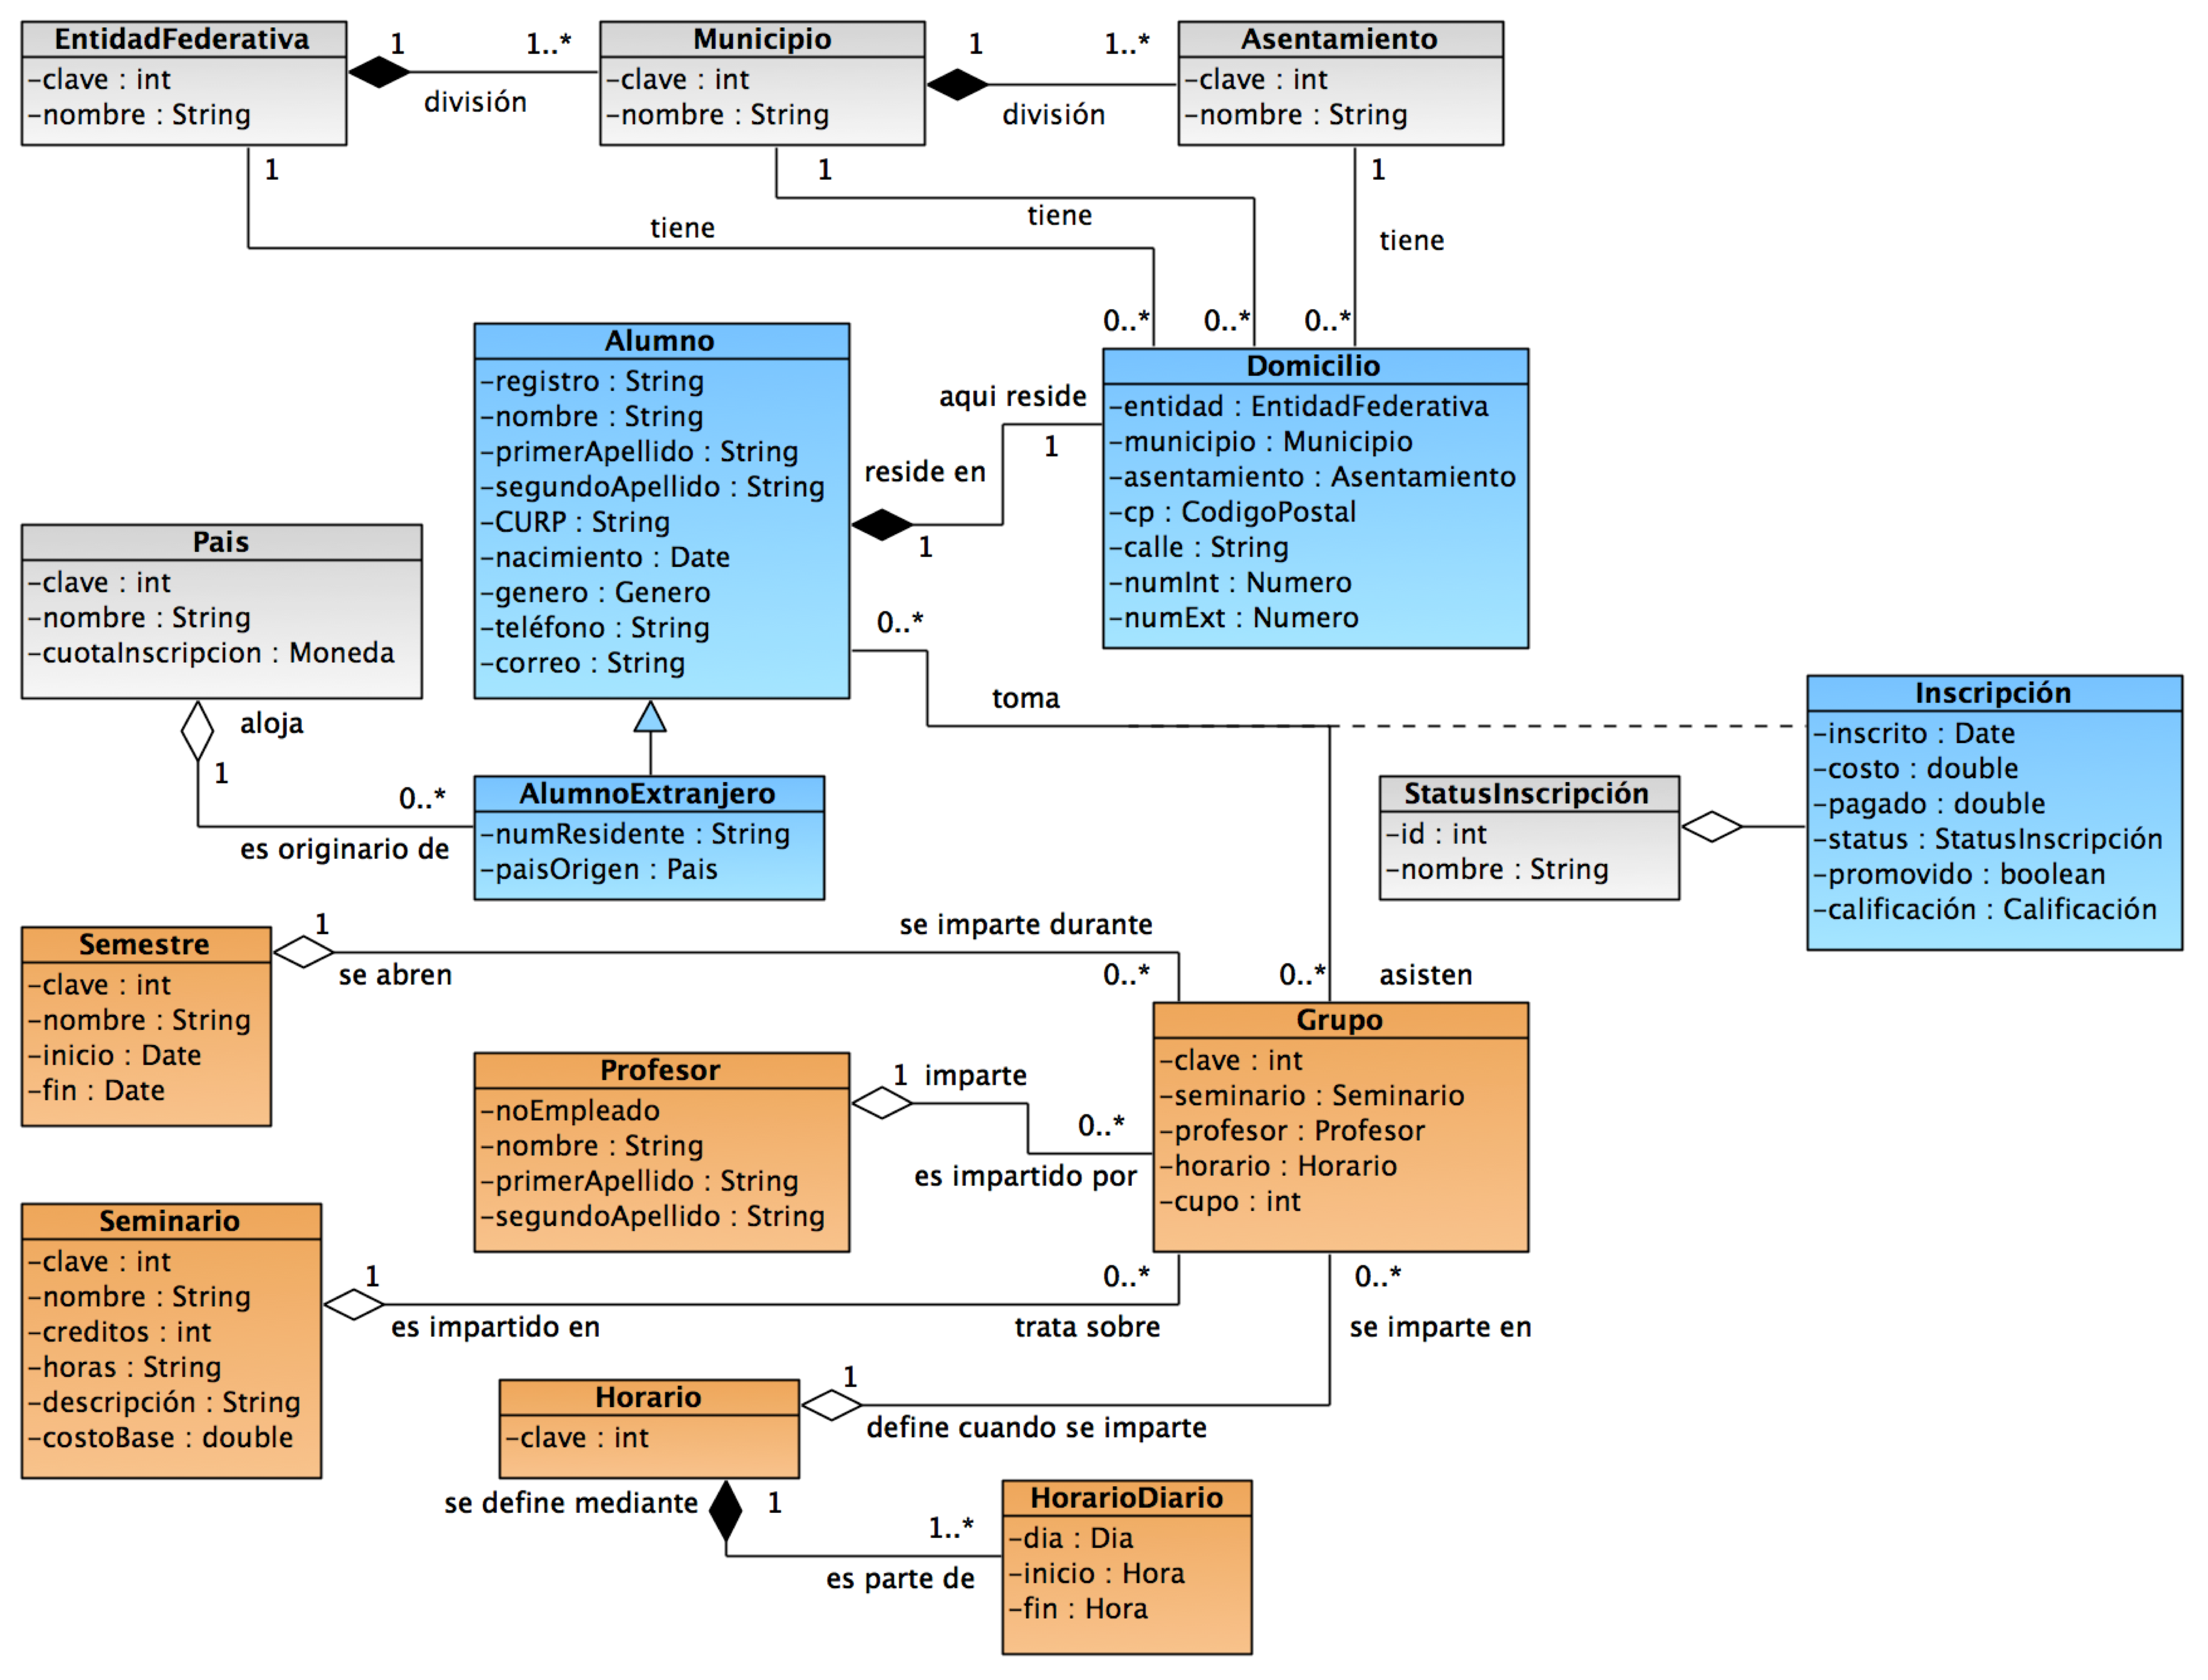
\includegraphics[angle=90,width=.95\textwidth]{images/modeloDelDominioDelProblema}
		\caption{Modelo del dominio del problema}
		\label{fig:modeloDeDominio}
	\end{center}
\end{figure}
